\section{Problem background} \label{sec:pb}

Augmented reality is an emerging technology, and it provides users with an interactive experience in both the physical and digital worlds. An augmented reality system aims at creating a real-time modification of the real-world environment for an interactive experience. Augmented reality continues to proliferate and become pervasive among a wide range of applications, including beauty. In the beauty industry, where live virtual try-on of beauty products is of great importance, augmented reality involves overlaying visual information onto real scenes so that not only user’s experience enhances, but companies also promote their products. To advance this domain, the segmentation task plays a key role.
\par
Semantic image segmentation, the task of mapping each pixel to a label, is a major and old challenge in the area of computer vision. Image segmentation can be treated as pixel-level prediction because it classifies each pixel into its category. With hair, segmentation problem strives for even fine details of strands of hair and avoid confusion between skin and hair. In the clothes segmentation problem, the output is a semantic analysis showing which clothing items are present, where in the image these are, and what shape they have.

\begin{figure} [H]
    \centering
    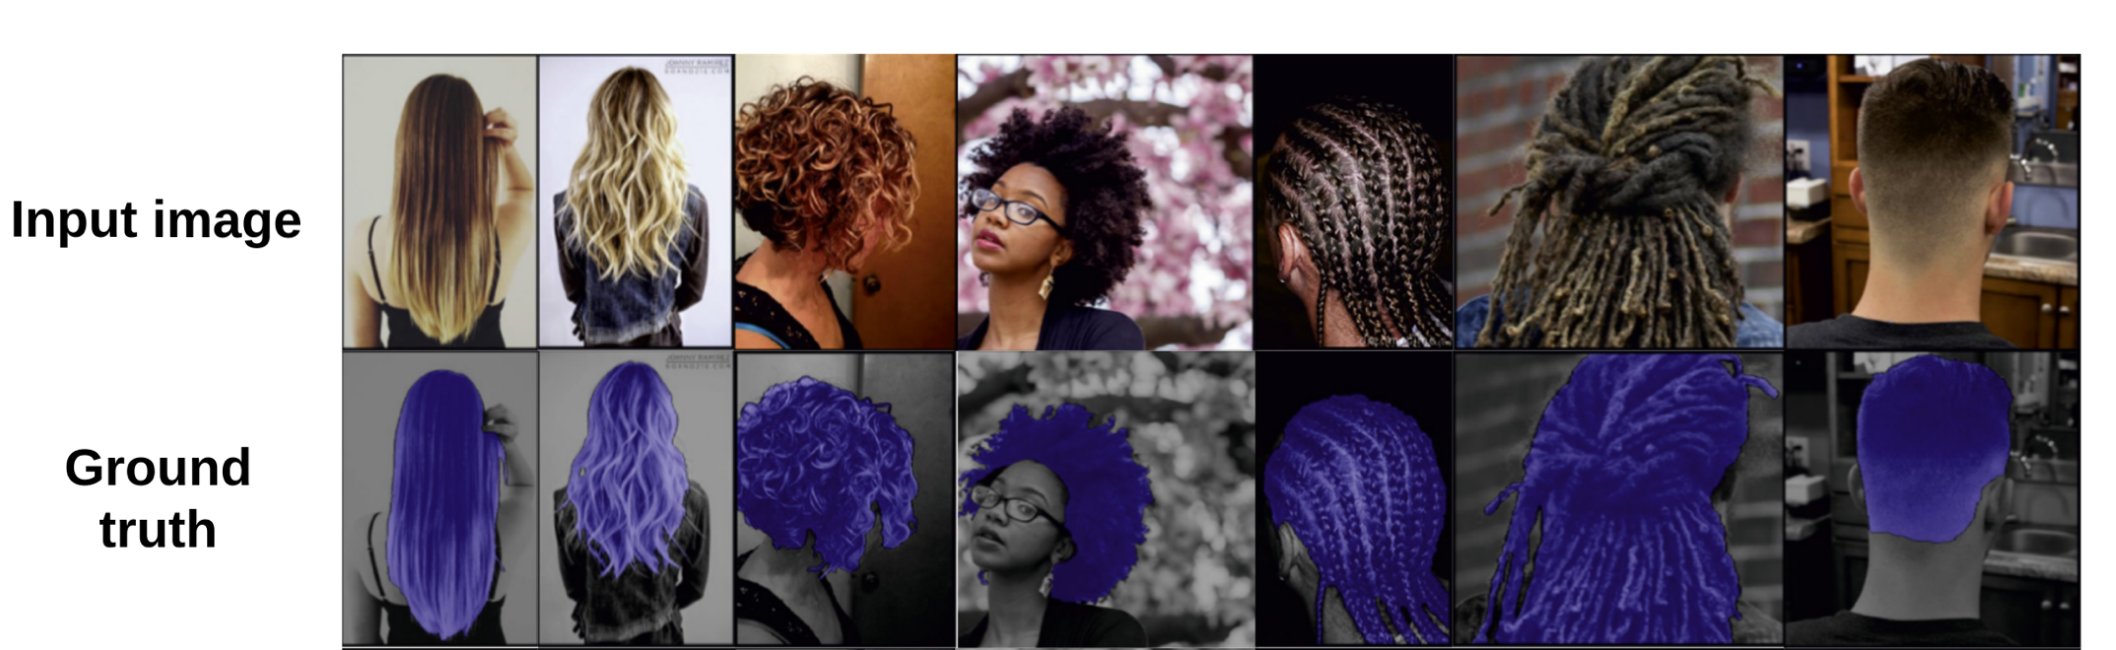
\includegraphics[width=0.9\textwidth]{chapter1/image/hair seg.png}
    \caption{Illustration for hair segmentation task. Hair masks is blue in color.}
    \label{fig:c1hairseg}
\end{figure}

With deep learning applied, this problem has been on the way to get an advanced performance in understanding image data. In addition to accuracy, the extent of media has also been extended to cover not just 2D images but also 3D images, videos, and so on. Apart from that, the field of deep learning possesses active communities and professional support. Tools for developing deep learning applications, such as Tensorflow, PyTorch, Caffe, were built in a modular way with a thorough document that makes development and engineering much more efficient. 
\par

Prior to the deep learning revolution, traditional image processing algorithms were used for both hair and clothes segmentation, but with deep learning, features are obtained automatically. Recent DNNs for hair segmentation are FPN \cite{fpn}, DenseNet \cite{densenet}, DeepLabv3 \cite{deeplabv3}. Aside from architecture, a hair matting technique utilizing image gradient is introduced in \cite{hairseg2matting}, playing the role of an auxiliary loss. Researchers also make an effort to apply filters to treat coarse masks \cite{hairseg2matting}. About clothing segmentation problem, Mask R-CNN \cite{maskrcnn}, Match R-CNN \cite{deepfashion2} are proposed to achieve instance segmentation in spite of complex architecture. The thesis work will exploit the start-of-the-art solution for hair and cloth segmentation tasks to achieve the thesis's goals. 
\par
\paragraph{Problem of real-time segmentation on mobile devices}

DNNs for segmentation are complex and require high memory usage and computational resources. Therefore, the main platforms to run these models must have a powerful computational unit (e.g., GPU support) or cloud. For instance, mobile applications often send input and receive output from Firebase, where developers push their DNNs. However, researchers recently realize the benefits of bringing deep learning toward the edge that includes devices with less power and resources. It ranges from user experience, offering anytime, anywhere access, with the great advantages of security, privacy, and energy consumption. \par

Discovering advantages from running DNNs on edge, big technology companies have been developing more and more frameworks to deploy models locally. A few must-mentioned frameworks for deep learning on mobile phones are TFLite, OONX, CoreML, PyTorch Mobile. Almost all frameworks for smartphones concern about optimization level, binary size, and supported hardware. Take the QNNPACK library \cite{qnnpack} for example, it is a mobile-optimized library for low-precision high-performance neural network inference. QNNPACK also provides the implementation of common neural network operators on quantized 8-bit tensors. Moreover, models developed especially for mobile also raise in the number; some of them are introduced in \textbf{section \ref{sec:cnn}}. 



